\clearpage
% start with Diamond sponsor on odd (right) page
% such that all Platinum sponsors appear on two
% adjacent / facing pages
\ifodd\value{page}\else\hbox{}\newpage\fi

\centering

% Diamond: Facebook

\incgraph[paper=document,options={width=105mm}]{ads/facebook.pdf}

% Platinum 

\incgraph[paper=document,a6paper]{ads/elsevier.pdf}

\incgraph[paper=document,options={width=120mm},a6paper]{ads/microsoft.pdf}

\incgraph[paper=document,options={width=120mm},a6paper]{ads/oracle.pdf}

\incgraph[paper=document,options={width=105mm},a6paper]{ads/tableau.pdf}

% Gold


\includegraphics[height=.49\textheight,width=\textwidth,keepaspectratio]{ads/alibaba.jpg}
\vfill

\includegraphics[height=.49\textheight,width=\textwidth,keepaspectratio]{ads/amazon.jpg}
\pagebreak


\includegraphics[height=.49\textheight,width=\textwidth,keepaspectratio]{ads/baidu.jpg}
\vfill

\includegraphics[height=.49\textheight,width=\textwidth,keepaspectratio]{ads/couchbase.eps}
\pagebreak


\includegraphics[height=.49\textheight,width=\textwidth,keepaspectratio]{ads/databricks.eps}
\vfill

\includegraphics[height=.49\textheight,width=\textwidth,keepaspectratio]{ads/google.eps}
\pagebreak

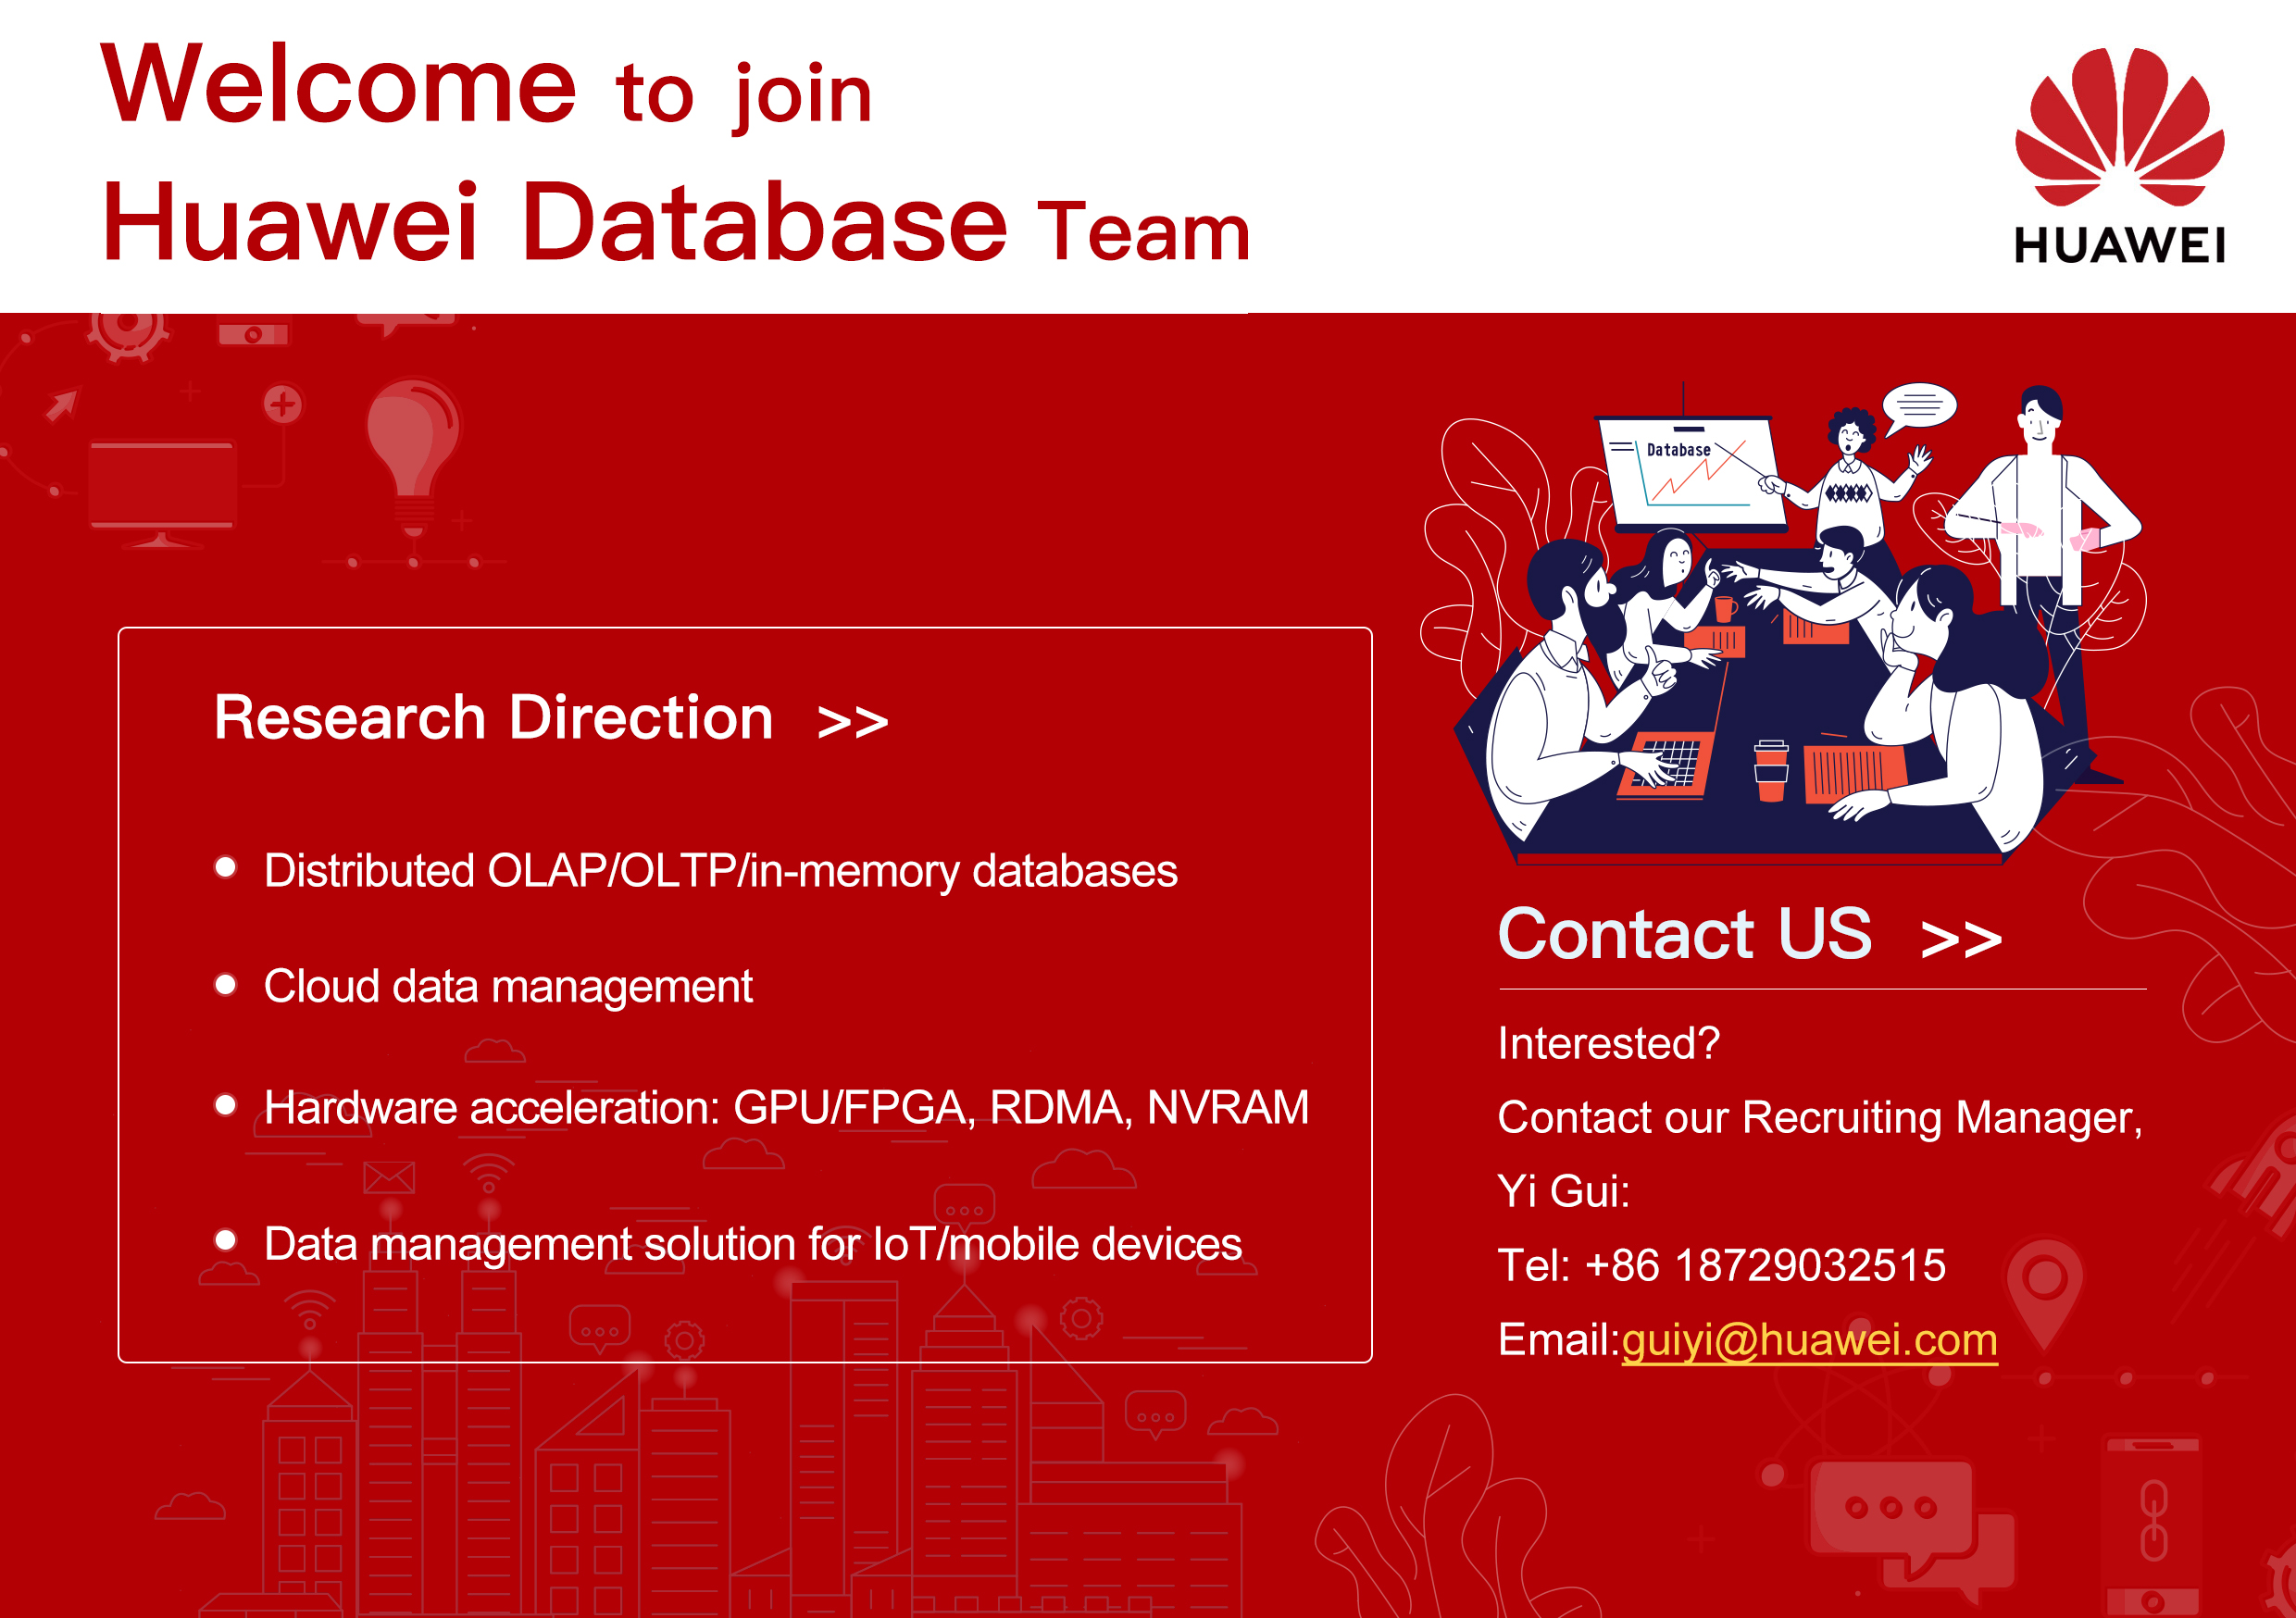
\includegraphics[height=.49\textheight,width=\textwidth,keepaspectratio]{ads/huawei.jpg}
\vfill

\includegraphics[height=.49\textheight,width=\textwidth,keepaspectratio]{ads/ibm.pdf}
\pagebreak


\includegraphics[height=.49\textheight,width=\textwidth,keepaspectratio]{ads/intel.jpg}
\vfill

\includegraphics[height=.49\textheight,width=\textwidth,keepaspectratio]{ads/megagon-cropped.pdf}
\pagebreak


\includegraphics[height=.49\textheight,width=\textwidth,keepaspectratio]{ads/monetdb.png}
\vfill
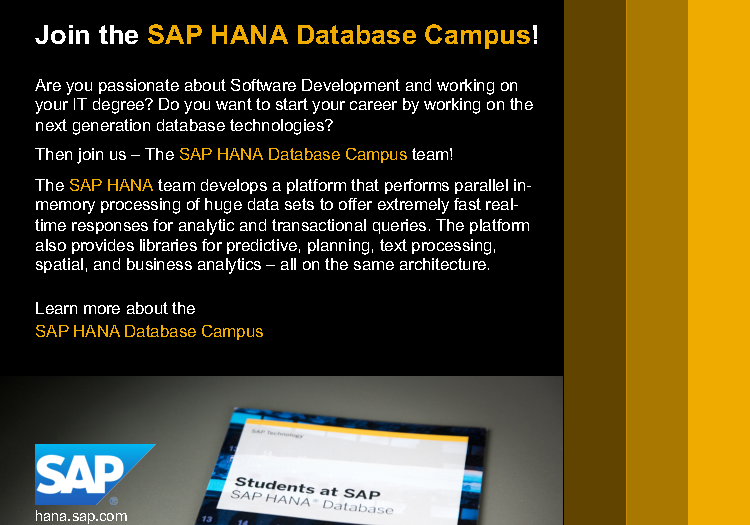
\includegraphics[height=.49\textheight,width=\textwidth,keepaspectratio]{ads/sap.pdf}
\pagebreak

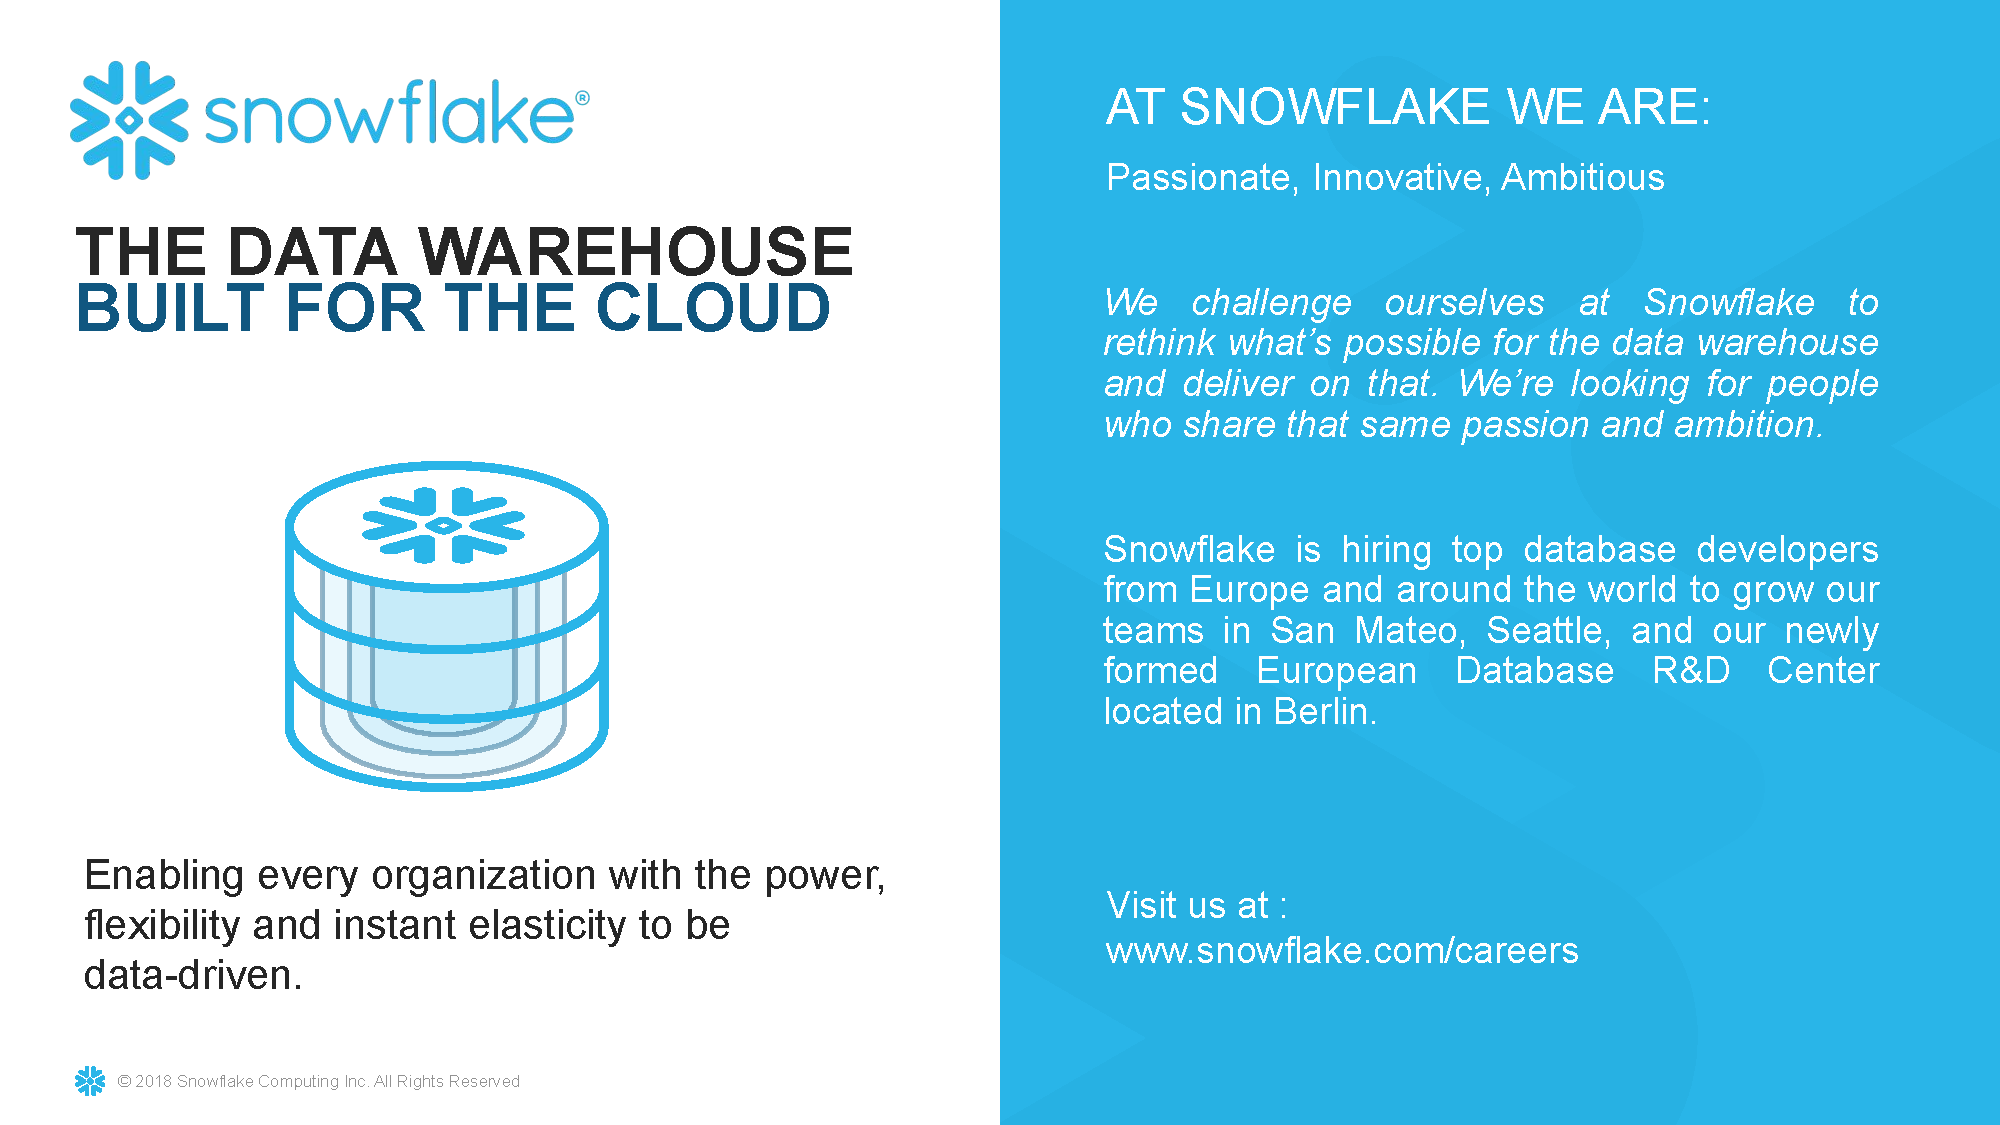
\includegraphics[height=.49\textheight,width=\textwidth,keepaspectratio]{ads/snowflake.pdf}
\vfill
%\includegraphics[height=.49\textheight,width=\textwidth,keepaspectratio]{ads/apple.pdf}
\pagebreak

% Silver

%% landscape
\ifodd\value{page}
$\vcenter{\hbox{
\includegraphics[keepaspectratio,width=.49\textheight,height=.49\textwidth,angle=90]{ads/mongodb.pdf}}}$
\hfill
$\vcenter{\hbox{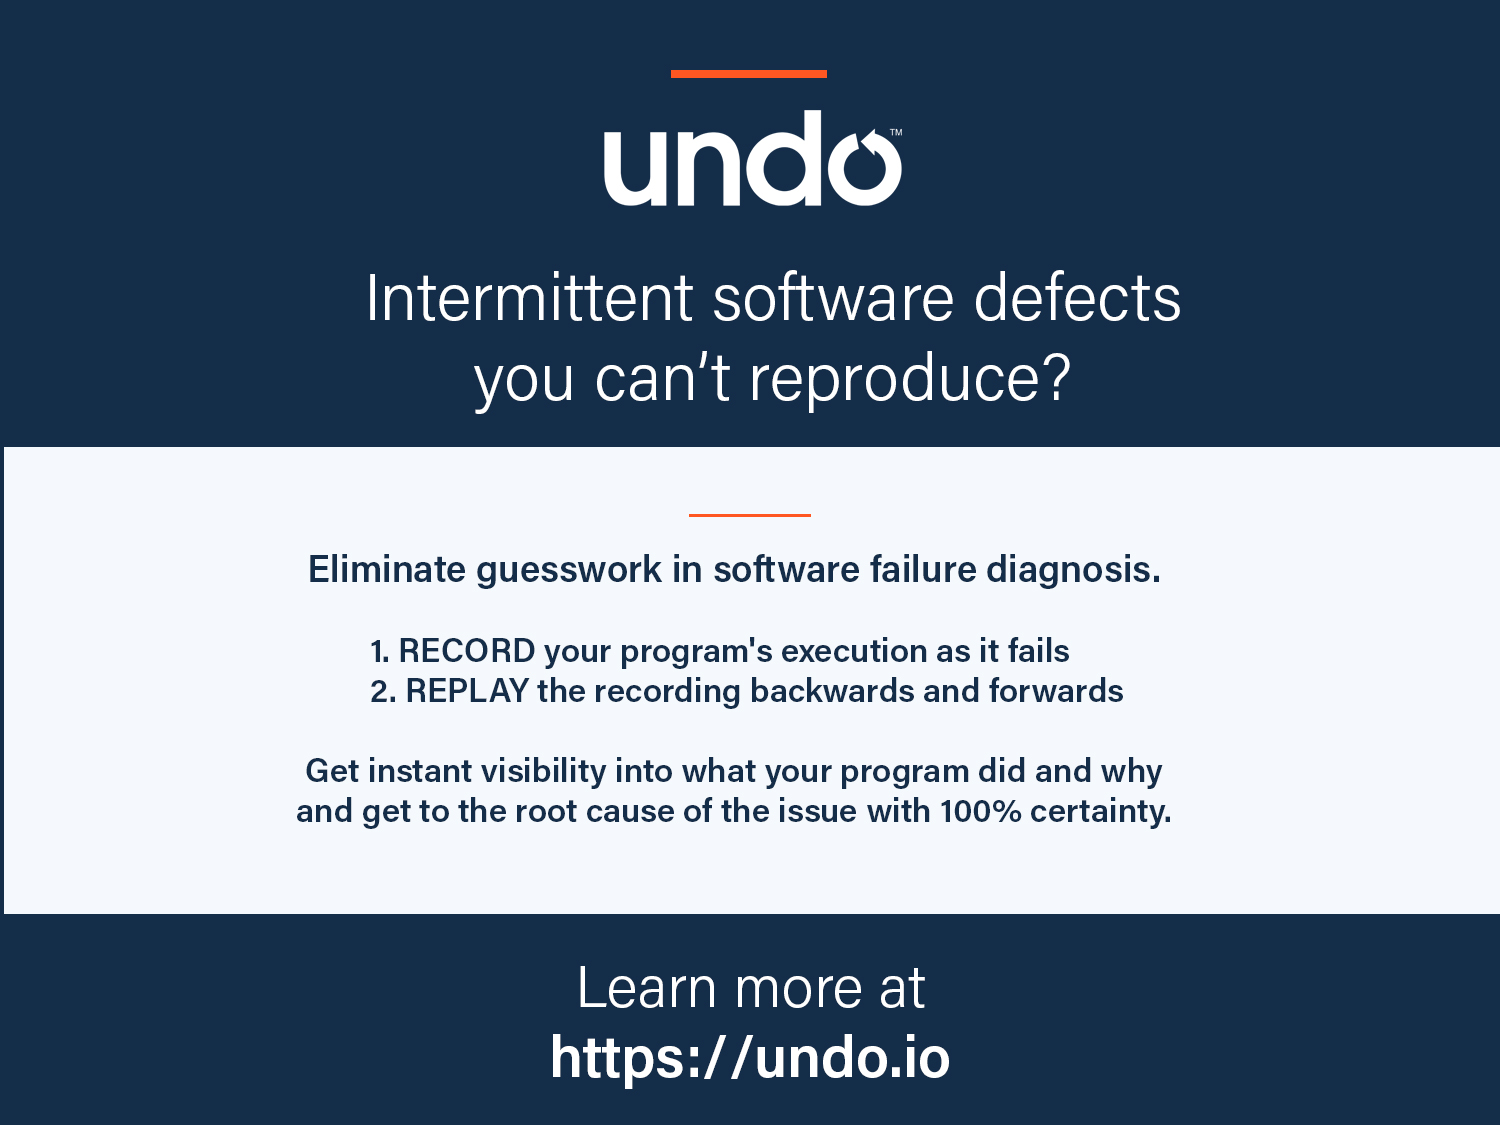
\includegraphics[keepaspectratio,width=.49\textheight,height=.49\textwidth,angle=90]{ads/undo.jpg}}}$
\vfill
$\vcenter{\hbox{
\includegraphics[keepaspectratio,width=.49\textheight,height=.49\textwidth,angle=90]{ads/ebay.png}}}$
\hfill
$\vcenter{\hbox{
\includegraphics[keepaspectratio,width=.49\textheight,height=.49\textwidth,angle=90]{ads/tigergraph.eps}}}$
\else
$\vcenter{\hbox{
\includegraphics[keepaspectratio,width=.49\textheight,height=.49\textwidth,angle=270]{ads/tigergraph.eps}}}$
\hfill
$\vcenter{\hbox{
\includegraphics[keepaspectratio,width=.49\textheight,height=.49\textwidth,angle=270]{ads/ebay.png}}}$
\vfill
$\vcenter{\hbox{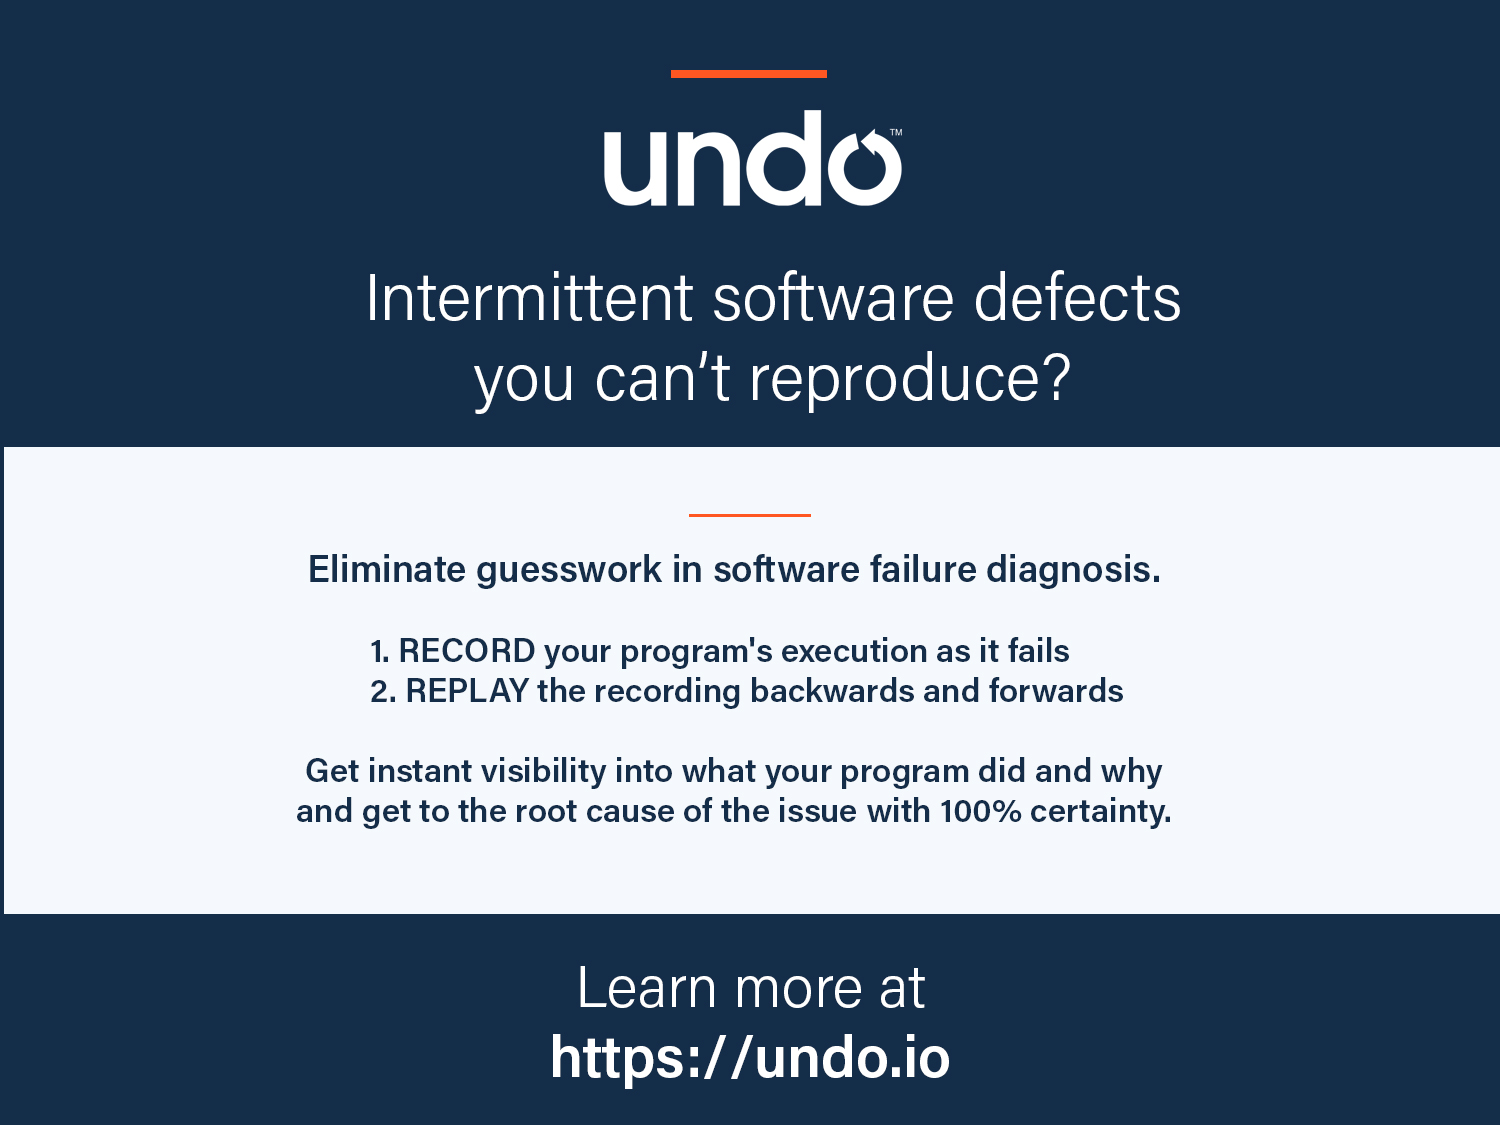
\includegraphics[keepaspectratio,width=.49\textheight,height=.49\textwidth,angle=270]{ads/undo.jpg}}}$
\hfill
$\vcenter{\hbox{
\includegraphics[keepaspectratio,width=.49\textheight,height=.49\textwidth,angle=270]{ads/mongodb.pdf}}}$
\fi
\pagebreak

%% portrait
$\vcenter{\hbox{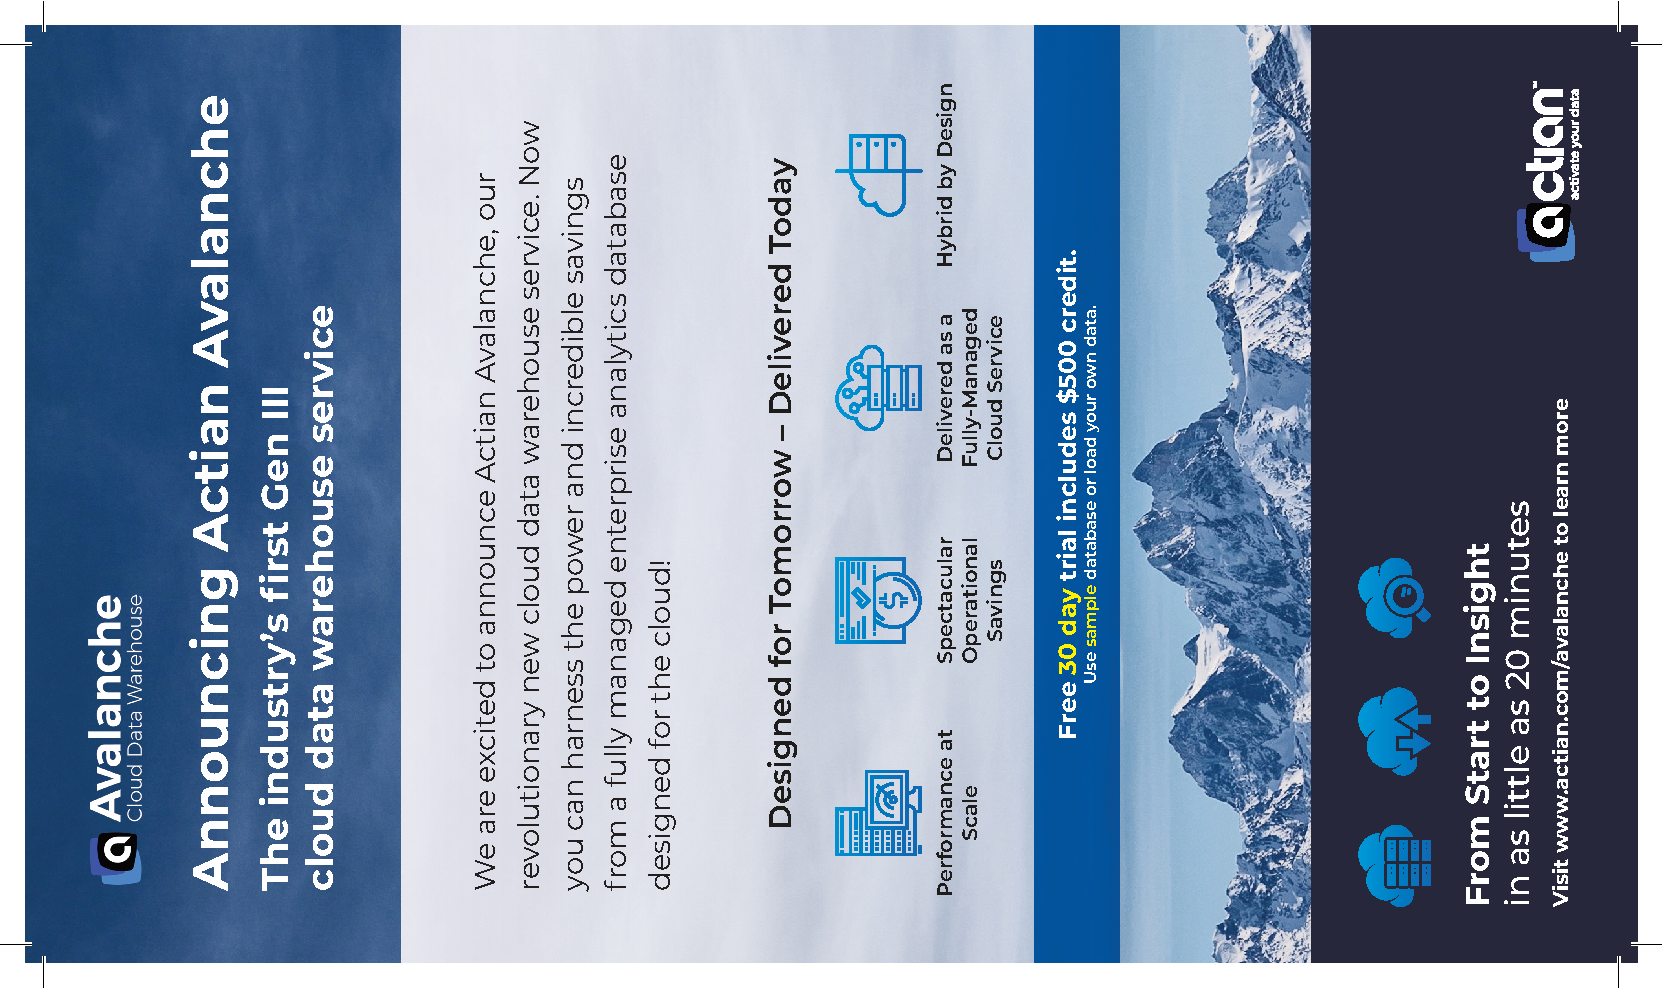
\includegraphics[keepaspectratio,width=.49\textheight,height=.49\textwidth,angle=270]{ads/actian.pdf}}}$
\hfill
~
\vfill
~
\hfill
~
\pagebreak





% % Google
% \begin{sloppypar}
% \begin{ssmall}
% 
\includegraphics[width=\linewidth]{ads/Google_Cover_Photo.png}

% \vspace{2mm}
% {\footnotesize{\textbf{Software Engineer, Infrastructure}}} \\
% Google \\
% Software Engineering

% \vspace{3mm}
% 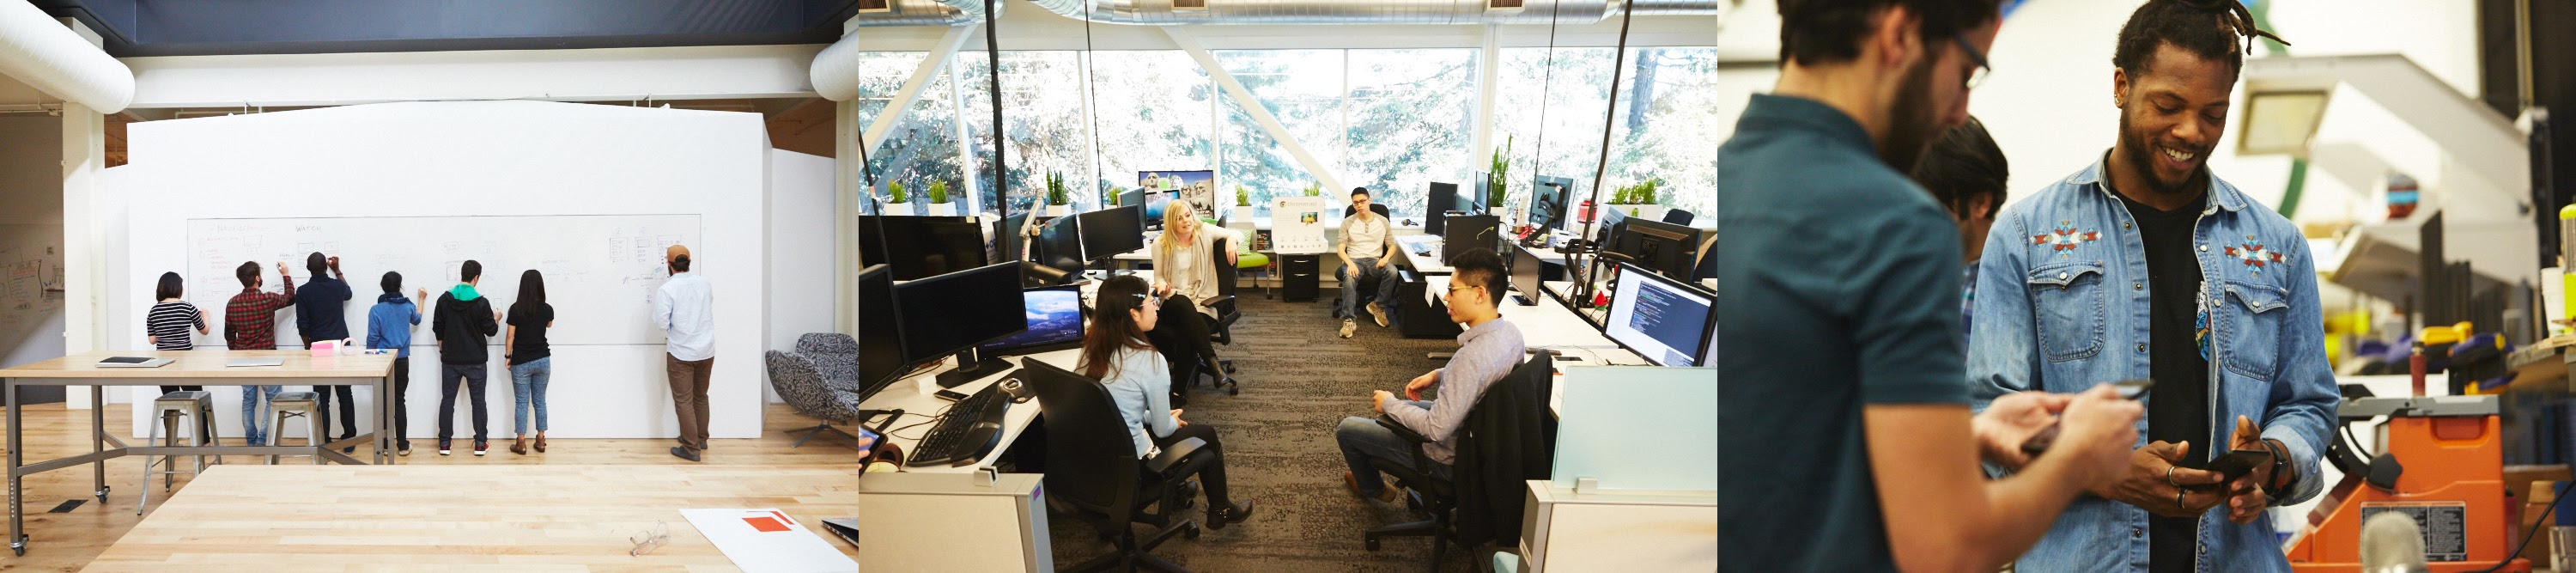
\includegraphics[width=\linewidth]{ads/Google_Pictures.png}

% Google's software engineers develop the next-generation technologies that change how billions of users connect, explore, and interact with information and one another. Our products need to handle information at massive scale, and extend well beyond web search. We're looking for engineers who bring fresh ideas from all areas, including information retrieval, distributed computing, large-scale system design, networking and data storage, security, artificial intelligence, natural language processing, UI design and mobile; the list goes on and is growing every day. As a software engineer, you will work on a specific project critical to Google’s needs with opportunities to switch teams and projects as you and our fast-paced business grow and evolve. We need our engineers to be versatile, display leadership qualities and be enthusiastic to tackle new problems across the full-stack as we continue to push technology forward.

 

% As a Software Engineer working on Google's infrastructure, you have the opportunity to work on everything from the core platform that runs the world's largest distributed network to redefining the systems that allow applications and services to provide useful information to billions of users around the globe. From our Data Center software groups to Google's Cloud Platform, Gmail to YouTube, our infrastructure engineers across departments wrestle with the vast scale of a ubiquitous system, its products, and services and revolutionize industry leading technologies to handle the sheer magnitude at which Google operates.

 
% \pagebreak
% Google is and always will be an engineering company. We hire people with a broad set of technical skills who are ready to tackle some of technology's greatest challenges and make an impact on millions, if not billions, of users. At Google, engineers not only revolutionize search, they routinely work on massive scalability and storage solutions, large-scale applications and entirely new platforms for developers around the world. From AdWords to Chrome, Android to YouTube, Social to Local, Google engineers are changing the world one technological achievement after another.


% \vspace{1mm}
% Responsibilities

% \begin{itemize}
% \setlength\itemsep{0mm}
% \item Build our platforms, systems and infrastructure using your strong background in distributed systems and large scale storage systems.
% \item Manage individual projects priorities, deadlines and deliverables with your technical expertise.
% \item Design, develop, test, deploy, maintain, and enhance software solutions.
% \end{itemize}

% Qualifications

% Minimum qualifications:

% \begin{itemize}
% \setlength\itemsep{0mm}
% \item BA/BS degree in Computer Science or related technical field or equivalent practical experience.
% \item 4 years of relevant work experience, including software development experience, or 1 year of relevant work experience with a PhD in Computer Science or related technical field.
% \item Professional coding experience in C/C++, Java, Python or Go.
% \item  Experience architecting and developing large scale distributed systems. Experience in concurrency, multithreading and synchronization.
% \end{itemize}
 

% Preferred qualifications:

% \begin{itemize}
% \setlength\itemsep{0mm}
% \item MS or PhD in Computer Science.
% \item Experience with Unix/Linux environments.
% \item Experience with TCP/IP and network programming.
% \item Experience with database internals, database language theories, database design, SQL and database programming.
% \item Understanding of technologies such as virtualization and global infrastructure, load balancing, networking, massive data storage, Hadoop, MapReduce and security.
% \item Interest or exposure to networking technologies/concepts such as Software Defined Networking (SDN) and OpenFlow.
% \end{itemize}

% %\href{https://careers.google.com/jobs?utm_source=Online&utm_medium=University_Board&utm_campaign=DIA_SWE&src=Online/Self%20Reported/DIA_SWE#!t=jo&jid=/google/software-engineer-infrastructure-1600-amphitheatre-pkwy-mountain-view-ca-212910046&}{link}

% \end{ssmall}
% \end{sloppypar}

% % Microsoft

% \incgraph[paper=document,options={width=105mm}]{ads/VLDB17_Anzeige_Microsoft_PLATINUM_left.pdf}
% \incgraph[paper=document,options={width=105mm}]{ads/VLDB17_Anzeige_Microsoft_PLATINUM_right.pdf}

% % Oracle

% \incgraph[paper=document,options={width=105mm}]{ads/VLDB17_Anzeige_Oracle_1_PLATINUM_cropped.pdf}
% \incgraph[paper=document,options={width=105mm}]{ads/VLDB17_Anzeige_Oracle_2_PLATINUM_cropped.pdf}

% % Recruit

% \incgraph[paper=document,options={width=105mm}]{ads/VLDB17_Anzeige_Recruit_PLATINUM_1_gs.pdf}
% \incgraph[paper=document,options={width=105mm}]{ads/VLDB17_Anzeige_Recruit_PLATINUM_2_gs.pdf}

% % Tableau

% \incgraph[paper=document,options={width=105mm}]{ads/VLDB17_Anzeige_Tableau_left_PLATINUM_NEW.pdf}
% \incgraph[paper=document,options={width=105mm}]{ads/VLDB17_Anzeige_Tableau_right_PLATINUM_NEW.pdf}

% % Teradata

% \incgraph[paper=document,options={width=105mm}]{ads/VLDB17_Anzeige_Teradata_PLATINUM_left_gs.pdf}
% \incgraph[paper=document,options={width=105mm}]{ads/VLDB17_Anzeige_Teradata_PLATINUM_right_gs.pdf}

% %%% Gold sponsors

% % Amazon: no show

% % Alibaba

% \incgraph[paper=document,options={width=105mm}]{ads/VLDB17_Anzeige_Alibaba-inc_GOLD.pdf}

% % facebook

% \incgraph[paper=document,options={width=105mm}]{ads/VLDB17_Anzeige_Facebook_GOLD.pdf}

% % Huawei

% \incgraph[paper=document,options={width=105mm}]{ads/VLDB17_Anzeige_Huawei_GOLD_fonts.pdf}

% % IBM

% \newpage
% \incgraph[paper=document,options={width=105mm}]{ads/VLDB17_Anzeige_IBM_GOLD_cropped.pdf}

% % SAP

% \incgraph[paper=document,options={width=105mm}]{ads/VLDB17_Anzeige_SAP_GOLD_fonts.pdf}

% %%% Silver sponsors

% \incgraph[paper=document,options={width=105mm}]{ads/silverpage1.pdf}

% \incgraph[paper=document,options={width=105mm}]{ads/silverpage2.pdf}
